\chapter{Implementation}
\label{sec:implementation}

% Hier greift man einige wenige, interessante Gesichtspunkte der
% Implementierung heraus. Das Kapitel darf nicht mit Dokumentation oder
% gar Programmkommentaren verwechselt werden. Es kann vorkommen, daß
% sehr viele Gesichtspunkte aufgegriffen werden müssen, ist aber nicht
% sehr häufig. Zweck dieses Kapitels ist einerseits, glaubhaft zu
% machen, daß man es bei der Arbeit nicht mit einem "Papiertiger"
% sondern einem real existierenden System zu tun hat. Es ist sicherlich
% auch ein sehr wichtiger Text für jemanden, der die Arbeit später
% fortsetzt. Der dritte Gesichtspunkt dabei ist, einem Leser einen etwas
% tieferen Einblick in die Technik zu geben, mit der man sich hier
% beschäftigt. Schöne Bespiele sind "War Stories", also Dinge mit denen
% man besonders zu kämpfen hatte, oder eine konkrete, beispielhafte
% Verfeinerung einer der in Kapitel 3 vorgestellten Ideen. Auch hier
% gilt, mehr als 20 Seiten liest keiner, aber das ist hierbei nicht so
% schlimm, weil man die Lektüre ja einfach abbrechen kann, ohne den
% Faden zu verlieren. Vollständige Quellprogramme haben in einer Arbeit
% nichts zu suchen, auch nicht im Anhang, sondern gehören auf Rechner,
% auf denen man sie sich ansehen kann.

\begin{itemize}

\item The CAL with Policy Based Design

  In section \ref{sec:cal} the CAL was introduced as an flexible
  Communication layer based on varying adapters. For the implementation
  of the varying adapters, a policy based design was choosen.

  % Policy based design in general
  A policy is a class or class template interface, which consists of
  inner type definitions, member functions and/or member variables. An
  implementation of a policy is called policy class and is inherited
  by or contained within a host class.
  The advantage of policy based design is that the varying
  functionality of the policy is bounded to its host class at compile
  time, providing no runtime overhead. And the interface of the policy
  is strictly defined by the host class. Ignoring this interface leads
  to errors at compile time.


  % Policy based design for CAL + adapter
  An adapter is the policy, here called communication policy, and the
  CAL is the host class (Figure \ref{fig:cal_uml}). The CAL takes an
  adapter as template argument and inheritates its properties in
  protected mode. 

  \begin{figure}[H]
    \centering 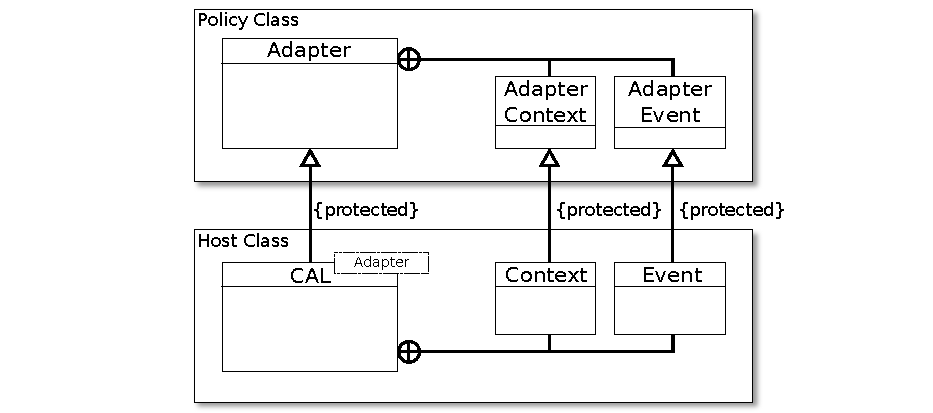
\includegraphics[width=\textwidth]{graphics/40_cal_uml}
    \caption{  }
    \label{fig:cal_uml}
  \end{figure}

  % Descrption Communication operations
  Usually, the adapter has to provide all communication and context
  operations discussed in section \ref{sec:cal_context} and
  \ref{sec:cal_comm}. But, policy based design has the characteristic
  that if a member function is missing in the policy and not used
  through the host class, the compiler will not throw an error. Thus
  only the used functions have to be implemented in an adapter (e.g
  just p2p functionality). But for sake of completeness an adapter
  should implement the whole policy interface.

  % Description Context + Event
  In addition to communication and context operations, the adapter has
  also to provide a inner context and a inner event class.  They
  contain the adapter specific implementations. The interface of these
  two inner classes is defined by similar inner classes of the CAL.

\item The MPI Adapter as Reference Implementation

  MPI (Section \ref{sec:mpi}) was as choosen existing communication
  layer for the reference adapter, because it already brings a lot of
  functionality required by the CAL interface. Additionally it is
  available on wide range of compute systems and can be used for free
  by open source implementations. The MPI C language binding is used
  in the adapter, because it is the most available implementation. An
  alternative would be the boost::mpi c++ implementation, which
  presupposes that beside a MPI implementation also the boost library
  is installed.

  Implementing the communication operation is straight forward, just a
  forwarding of arguments and a function call. More tricky is the
  support of abitrary binary operations for the reduce operation and
  the support of abitrary data types of the trasmitted data.

  \begin{itemize}
  \item Binary Function

    The binary functions that takes the CAL as argument for reduce 
    operations have to be translated to binary MPI operations.

    There exists two possible ways to do so. The easiest way, is that
    the MPI adapter provides all binary MPI functions by itself as
    kind of a struct with static const expressions (Listing
    \ref{lst:mpi_bin}). The reduce can for example be defined as
    BinaryOperations::MAX.

    \begin{lstlisting}[language=C++]
      struct BinaryOperations { 	
        static constexpr BinaryOperation MAX = MPI_MAX; 	
        static constexpr BinaryOperation MIN = MPI_MIN; 	
        static constexpr BinaryOperation SUM = MPI_SUM; 	
        static constexpr BinaryOperation PROD = MPI_PROD;
	...
      };
    \end{lstlisting}
    \label{lst:mpi_bin}

    The downside of the first approach is that only the predefined
    operations of MPI can be used. But is possible to use abitrary
    binary functions with MPI\_Op\_create. This can be done for all
    handed over binary operation from the CAL. The only requirement is
    that the binary operation has to be a struct like discussed in
    section \ref{sec:cal_collective}.  Because of more flexibility the
    second approach was choosen to implemend binary functions for the
    MPI adapter.

  \item  Data Type Conversion 

    MPI predefines on one hand its primitive data types, but on the
    other hand also provides facilities to define own data structures
    based upon sequences of the MPI promitive data types. Such user
    defined structures are called derived data types. Primitive data
    types are contiguous. Derived data types allow you to specify
    non-contiguous data in a convenient manner and to treat it as
    though it was contiguous.

    The primitive c++ data types can be mapped directly to primitive
    c++ data types. The conversation is implemented by c++ traits
    (Listing \ref{lst:mpi_trait}).  First, a generic template is
    defined that implements the default behaviour. In this case
    unknown types will assumed to be MPI\_CHAR. The second template is
    a specialisation for int, which will be transformed to MPI\_INT.


    \begin{lstlisting}[language=C++]
      template<typename T>
      struct MPIDatatypes{
	static constexpr MPI_Datatype type = MPI_CHAR;
      };

      template<>
      struct MPIDatatypes<int>{
    	static constexpr MPI_Datatype type = MPI_INT;
      };

    \end{lstlisting}
    \label{lst:mpi_trait}


    More complex data types (e.g structs or classes) have to be
    transformed into derived data types. These are not implemented
    until yet, but are allready available in the boost::mpi
    implementation. Thus switching to boost::mpi would solve this
    problem without any further effort.
    
  \item Context
  \item Event
  \end{itemize}

\item Graph Based on the Boost Graph Library

  % BGL as backend
  The graph introduced in section \ref{sec:graph} was not written
  from the scratch. There are a varity of libraries providing
  graph implementations. Because of the closeness of the boost
  library to the c++ STL, the boost graph library, short BGL, 
  was choosen. While the BGL provides a lot of functionality,
  just a small subset is really needed for the purposes of
  this library. Thus the BGL is wrapped inside a graph class
  just providing standard graph funcionality.

  \begin{itemize}  

  \item Vertices identified by Properties

    % Properties
    Like in section \ref{sec:graph} discussed, a graph has so called
    properties to describe its vertices and edges. These properties are
    configured at compile time and define vertices and edges itself. The
    properties are structs or classes with abitrary content. However
    these properties need to provide an unsigned id variable to create
    an internal binding of vertices to properties. 


    The BGL itself refers to vertices by integer numbers, whereby
    properties of this integer vertices can be queried. Here the
    vertices are represented by its property. Asking for the vertices of
    the graph, returns a vector of vertices, which is a list of vertex
    properties in the context of the BGL.
  
  \item Operations on the graph / vertices
    % Operations
    The graph provides simple graph operations like retrieving all
    vertices, retrieving adjacent vertices, retrieving in and out
    edges.


  \item Creation of subgraphs
    % Subgraph Createion
    Another reason for the BGL is the builtin subgraph support. The
    creation of subgraphs is meant to be used as an equivalent to the
    creation of contexts. Thus a subgraph can be created from its
    supergraph by a subset of its vertices. Collective operations on
    this subgraph only consider only vertices within this subgraph.

  
  \end{itemize}
  
\item Configuration of an Application by Templates
  \begin{itemize}
  \item Creation of a Graph
  \item Example Configuration of a Communication System
  \end{itemize}

\item Implementing a Game of Life
  \begin{itemize}
  \item Based on Cells
  \item Based on Bundles
  \end{itemize}

\end{itemize}




\cleardoublepage

%%% Local Variables:
%%% TeX-master: "diplom"
%%% End:
